\begin{inhalt}
\renewcommand*\chapterpagestyle{scrheadings}
\chapter{Datenbank}

In diesem Abschnitt werden die Struktur, verwendete Tabellen sowie die wichtigen SQL-Befehle, Trigger und Funktionen der Datenbank detailliert erläutert.

\section{Tabellen}

Die Datenbank besteht aus den folgenden Tabellen:

\subsection{Schule (Schools)}
Die Tabelle speichert Informationen zu den Schulen, einschließlich Standort und Webseite. Der Primärschlüssel (\texttt{id}) wird automatisch generiert.

\begin{lstlisting}[style=mysql]
CREATE TABLE schools (
    id UUID PRIMARY KEY DEFAULT gen_random_uuid(),
    created_at TIMESTAMPTZ DEFAULT now(),
    name TEXT,
    location JSONB,
    website_url TEXT
);
\end{lstlisting}

\subsection{Abteilungen (Departments)}
Die Tabelle verwaltet die verschiedenen Abteilungen innerhalb einer Schule. Jede Abteilung ist eindeutig einer Schule zugeordnet.

\begin{lstlisting}[style=mysql]
CREATE TABLE departments (
    id UUID PRIMARY KEY DEFAULT gen_random_uuid(),
    created_at TIMESTAMPTZ DEFAULT now(),
    name TEXT,
    school_id UUID REFERENCES schools(id)
);
\end{lstlisting}

\subsection{Klassen (Classes)}
Diese Tabelle speichert Informationen zu den Klassen, die spezifischen Abteilungen angehören.

\begin{lstlisting}[style=mysql]
CREATE TABLE classes (
    id UUID PRIMARY KEY DEFAULT gen_random_uuid(),
    created_at TIMESTAMPTZ DEFAULT now(),
    name TEXT,
    department_id UUID REFERENCES departments(id)
);
\end{lstlisting}

\subsection{Geräte (Sensors)}
Die Tabelle enthält Informationen zu den einzelnen Sensor-Geräten, welche jeweils einer Klasse  ist.

\begin{lstlisting}[style=mysql]
CREATE TABLE sensors (
    id UUID PRIMARY KEY DEFAULT gen_random_uuid(),
    name TEXT,
    created_at TIMESTAMPTZ DEFAULT now()
);
\end{lstlisting}

\subsection{Benutzerprofile (Profiles)}
In dieser Tabelle werden Benutzerdaten, Rollen und deren Zugehörigkeit zu Klassen verwaltet. Zudem sind hier Statusinformationen wie \texttt{approved} und \texttt{email\_confirmed\_at} gespeichert.

\begin{lstlisting}[style=mysql]
CREATE TABLE profiles (
    id UUID PRIMARY KEY DEFAULT gen_random_uuid(),
    created_at TIMESTAMPTZ DEFAULT now(),
    first_name TEXT,
    surname TEXT,
    username TEXT,
    role INTEGER,
    class_id UUID REFERENCES classes(id),
    email_confirmed_at TIMESTAMPTZ,
    approved BOOLEAN
);
\end{lstlisting}

\subsection{Trigger und Funktionen}

\textbf{handle\_new\_user}


Diese Funktion erstellt automatisch ein Benutzerprofil, sobald ein neuer Benutzer angelegt wird. Dies erleichtert die Verwaltung von Nutzerdaten.

\begin{lstlisting}[style=mysql]
CREATE OR REPLACE FUNCTION public.handle_new_user()
 RETURNS trigger
 LANGUAGE plpgsql
 SECURITY DEFINER
 SET search_path TO ''
AS $function$
begin
  insert into public.profiles (id)
  values (new.id);
  return new;
end;
$function$;
\end{lstlisting}

\vspace{0.75cm}

\textbf{handle\_updated\_email\_confirmed\_at}
Diese Funktion aktualisiert das Feld \texttt{email\_confirmed\_at} im Profil eines Benutzers, wenn die E-Mail-Adresse bestätigt wird. Dies gewährleistet die Synchronität zwischen Authentifizierungs- und Profiltabellen.

\begin{lstlisting}[style=mysql]
CREATE OR REPLACE FUNCTION public.handle_updated_email_confirmed_at()
 RETURNS trigger
 LANGUAGE plpgsql
 SECURITY DEFINER
 SET search_path TO ''
AS $function$
BEGIN
  IF NEW.email_confirmed_at IS DISTINCT FROM OLD.email_confirmed_at THEN
    UPDATE public.profiles
    SET email_confirmed_at = NEW.email_confirmed_at
    WHERE id = NEW.id;
  END IF;
  RETURN NEW;
END;
$function$;
\end{lstlisting}

Die Implementierung dieser Funktion erfolgt ebenfalls durch einen Trigger, welcher Änderungen in der Tabelle \texttt{auth.users} überwacht.

\newpage

\section{Storage}

Für die Avatar-Bilder wurde die \texttt{Storage}-Funktion von Supabase verwendet, um Bilder einfach abrufen und hochladen zu können.  
Hierfür wurde ein Bucket (oberster Ordner bzw. Container) mit dem Namen \texttt{Avatar} erstellt.

\begin{figure}[!htb]
\centering
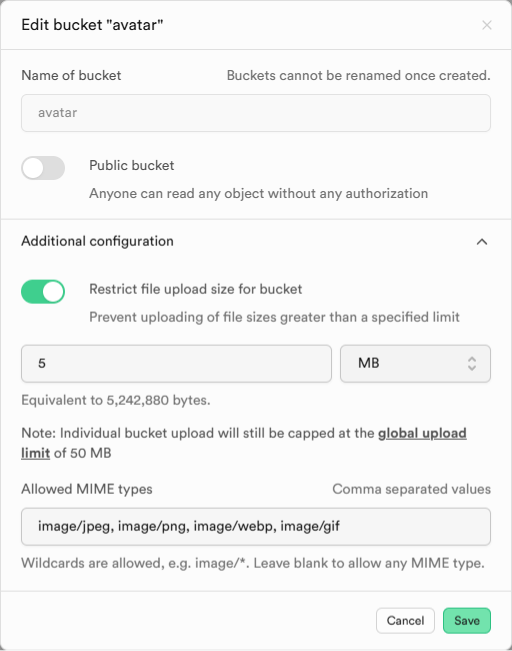
\includegraphics[width=0.55\textwidth]{files/Thomas/pics/Datenbank/storage/supabase_bucket_create.png}
\caption[Erstellen eines Buckets in Supabase]{Erstellen eines Buckets in Supabase}
\label{fig:supabase_bucket_create}
\end{figure}

Wie in Abbildung \ref{fig:supabase_bucket_create} zu sehen ist, wurde der Bucket so konfiguriert, dass nur Bilder mit einer maximalen Dateigröße von 5\,MB und ausschließlich Dateien im \texttt{image}- oder \texttt{gif}-Format hochgeladen werden dürfen.

Die Dateistruktur des Buckets ist wie folgt aufgebaut:

\begin{lstlisting}[style=mysql]
avatar/
 └── [user-id]/
      └── avatar.png
\end{lstlisting}

Somit kann jedem Benutzer ein individuelles Profilbild zugewiesen werden.

\newpage

\section{Auth}

Für die Authentifizierung wurde festgelegt, dass sich Benutzer mittels E-Mail und Passwort anmelden müssen.  
Bevor sich ein Benutzer jedoch anmelden darf, muss er zunächst seine E-Mail-Adresse verifizieren.  
Diese Funktion kann in den Supabase-Einstellungen aktiviert werden.  
Sobald ein Benutzer sich registriert, sendet Supabase automatisch eine Verifizierungs-E-Mail.

\begin{figure}[!htb]
\centering
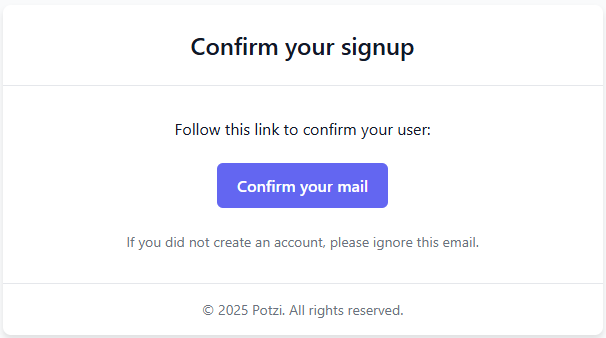
\includegraphics[width=0.75\textwidth]{files/Thomas/pics/Datenbank/auth/signup-email.png}
\caption[Supabase E-Mail-Verifizierung]{E-Mail-Verifizierung bei Supabase}
\label{fig:supabase_signup_email}
\end{figure}

Der Benutzer muss anschließend nur noch den Verifizierungslink in der E-Mail anklicken, um seine E-Mail-Adresse erfolgreich zu bestätigen.










\end{inhalt}